\subsection{Cryptosystem and Encryption Scheme}
\begin{itemize}
	\item A \textbf{cryptosystem} is the abstract formal definition encompassing all components necessary for secure communication.
	\item An \textbf{encryption scheme} specifies the algorithms (or protocols) used to implement encryption and decryption within a cryptosystem.
\end{itemize}
\vfill
\begin{figure}[h!]\centering
\begin{tikzpicture}[
	node distance=3cm and 4cm,
	box/.style={draw, rounded corners, minimum width=3cm, minimum height=1cm, align=center},
	arrow/.style={-Stealth, thick},
	prob/.style={draw, circle, inner sep=1pt, minimum size=1cm, align=center}
	]
	
	% Nodes
	\node[box] (plaintext) {\textbf{Plaintext} \\($\mathcal{P}$)};
	\node[box, below right=of plaintext, yshift=2cm] (encryption) {\textbf{Encryption} \\($\mathcal{E}$)};
	\node[box, above right=of encryption, yshift=-2cm] (ciphertext) {\textbf{Ciphertext} \\($\mathcal{C}$)};
	\node[box, above left=of ciphertext, yshift=-2cm] (decryption) {\textbf{Decryption} \\($\mathcal{D}$)};
	\node[box, right=of plaintext] (keyspace) {\textbf{Keyspace} \\($\mathcal{K}$)};
	
	% Connections
%	\draw[arrow, out=-90, in=180] (plaintext) to node[midway, above] {$p$} (encryption);
%	\draw[arrow, out=0, in=-90] (encryption) to node[midway, above] {$c$} (ciphertext);
%	\draw[arrow, out=90, in=0] (ciphertext) to node[midway, above] {$c$} (decryption);
%	\draw[arrow, out=-45, in=45] (keyspace) to node[midway, right] {$k$} (encryption);
%	\draw[arrow, out=135, in=225] (keyspace) to node[midway, left] {$k$} (decryption);
%	\draw[arrow, out=180, in=90] (decryption) to node[midway, above] {$p$} (plaintext);

	\draw[arrow] (plaintext) to node[midway, above] {$p$} (encryption);
	\draw[arrow] (encryption) to node[midway, above] {$c$} (ciphertext);
	\draw[arrow] (ciphertext) to node[midway, above] {$c$} (decryption);
	\draw[arrow] (keyspace) to node[midway, right] {$k$} (encryption);
	\draw[arrow] (keyspace) to node[midway, left] {$k$} (decryption);
	\draw[arrow] (decryption) to node[midway, above] {$p$} (plaintext);
\end{tikzpicture}
\caption{Cryptosystem}
\end{figure}
\vfill
\begin{figure}[h!]
\begin{tikzpicture}[
	node distance=3cm and 4cm,
	box/.style={draw, rounded corners, minimum width=3cm, minimum height=1cm, align=center},
	redbox/.style={draw, rounded corners, minimum width=3cm, minimum height=1cm, align=center, fill=red!10},
	arrow/.style={-Stealth, thick},
	prob/.style={draw, circle, inner sep=1pt, minimum size=1cm, align=center}
	]
	
	% Nodes
	\node[box] (plaintext) {\textbf{Plaintext} \\ ($\mathcal{P}$)};
	\node[redbox, below right=of plaintext, yshift=2cm] (enc) {\textbf{Encryption} \\ ($\enc$)};
	\node[box, above right=of encryption, yshift=-2cm] (ciphertext) {\textbf{Ciphertext} \\ ($\mathcal{C}$)};
	\node[redbox, above left=of ciphertext, yshift=-2cm] (dec) {\textbf{Decryption} \\ ($\dec$)};
	\node[redbox, right=of plaintext] (keygen) {\textbf{Key Generation} \\ ($\keygen$)};
	
	% Connections
	\draw[arrow] (keygen) to node[midway, right] {$k$} (enc);
	\draw[arrow] (keygen) to node[midway, left] {$k$} (dec);
	\draw[arrow] (plaintext) to node[midway, above] {$p$} (enc);
	\draw[arrow] (enc) to node[midway, above] {$c$} (ciphertext);
	\draw[arrow] (ciphertext) to node[midway, above] {$c$} (dec);
	\draw[arrow] (dec) to node[midway, above] {$p$} (plaintext);
\end{tikzpicture}
\caption{Encryption Scheme}
\end{figure}

\newpage
\defbox[Cryptosystem]{\begin{definition}
	A \textbf{cryptosystem} is a five-tuple \[
	(\plaintext,\ciphertext,\keyspace,\encryption,\decryption),
	\] where \begin{enumerate}[(i)]
		\item $\boxed{\plaintext}$ is a finite set of all possible plaintexts\footnote{These are the possible inputs to the encryption algorithm and typically represent meaningful data to be protected.}.
		\item $\boxed{\ciphertext}$ is a finite set of all possible  ciphertexts\footnote{These are the encrypted outputs of the encryption algorithm corresponding to plaintexts in $\plaintext$.}. 
		\item $\boxed{\keyspace}$ is a finite set of all possible keys\footnote{Each key $k\in\keyspace$ determines a specific encryption and decryption function.}. 
		\item $\boxed{\encryption:\keyspace\times\plaintext\to\ciphertext}$ is a deterministic function that maps a key 
		$k\in\keyspace$ and a plaintext $p\in\plaintext$ to a ciphertext $c\in\ciphertext$. Formally:
		\[
		\fullfunction{\encryption}{\keyspace\times\plaintext}{\ciphertext}{(k,p)}{c}.
		\]
		\item $\boxed{\decryption:\keyspace\times\ciphertext\to\plaintext}$ is a deterministic function that maps a key 
		$k\in\keyspace$ and a ciphertext $c\in\ciphertext$ to a ciphertext $p\in\plaintext$. Formally:
		\[
		\fullfunction{\decryption}{\keyspace\times\ciphertext}{\plaintext}{(k,c)}{p}.
		\]
	\end{enumerate}
\end{definition}}
\begin{remark}[Correctness Property]
	For every key $k\in\keyspace$ and every plaintext $p\in\plaintext$, the decryption function is the inverse of the encryption function. That is: \[
	\decryption(k,\encryption(k,p))=p.
	\]
\end{remark}
\begin{remark}[Security]
	The security of the cryptosystem is defined with respect to a particular adversarial model. Informally, a cryptosystem is secure if an adversary with limited computational resources cannot distinguish between the ciphertexts of any two plaintexts, even if they know the encryption algorithm but do not know the key.
\end{remark}
\vfill
\defbox[Encryption Scheme]{\begin{definition}
	An \textbf{encryption scheme} is a three-tuple \[
	\Pi:=(\keygen,\enc,\dec).
	\] where \begin{enumerate}[(i)]
		\item $\keygen$ is a probabilistic algorithm that ouputs a key $k\in\keyspace$, where $\keyspace$ is the key space. Formally: \[
		\boxed{\keygen:\set{0,1}^*\to\keyspace},
		\] where $\set{0,1}^*$ is the set of binary strings of arbitrary length (representing randomness or input seed). The ouput $k$ is uniformly distributed over $\keyspace$.
		\item $\enc$ is a (possibly probabilistic) algorithm that takes a key $k\in\keyspace$ and a message $p\in\messagespace$ (message space) and outpus a ciphertext $c\in\ciphertext$ (ciphertext sapce). Formally: \[
		\boxed{\enc:\keyspace\times\messagespace\ \textcolor{gray!50}{\times\set{0,1}^*}\to\ciphertext}.
		\] The algorithm may use randomness (from $\set{0,1}^*$) to ensure that repeated encryptions of the same message $m\in\messagespace$ under the same key $k\in\keyspace$ yield different ciphertexts 
		$c$.
		\item $\dec$ is a deterministic algorithms that takes a key $k\in\keyspace$ and a ciphertext $c\in\ciphertext$ and ouputs the corresponding message $m\in\messagespace$. Formally: \[
		\boxed{\dec:\keyspace\times\ciphertext\to\messagespace}.
		\]
	\end{enumerate}
\end{definition}}
\begin{remark}[Correctness Property]
For every $k\in\keyspace$, $m\in\messagespace$, and $c\in\ciphertext$, the scheme must satisfy \[
\dec(k,\enc(k,m; r))=m
\] where $r$ represents the random bits used by $\enc$.
\end{remark}
\begin{remark}[Security]
	The security of an encryption scheme depends on the adversarial model. For \textbf{semantic security}, an encryption scheme must satisfy the following:
	\begin{quote}
		``Given a ciphertext $c$, no computationally bounded adversary can distinguish between encryptions of any two messages $m_0,m_1$, even if they are chosen adaptively by the adversary.''
	\end{quote}
\end{remark}
\vspace{40pt}
\begin{example}[IND-CPA]
\ \\ The \textbf{indistinguishability under chosen plaintext attack (IND-CPA)} model: \begin{enumerate}[1.]
	\item The adversary chooses two messages $m_0,m_1$.
	\item A random bit $b\in\set{0,1}$ is chosen, and the ciphertext $c=\enc(k,m_b)$ is provided to the adversary.
	\item The adversary outputs a guess $b'\in\set{0,1}.$
\end{enumerate}
\begin{center}
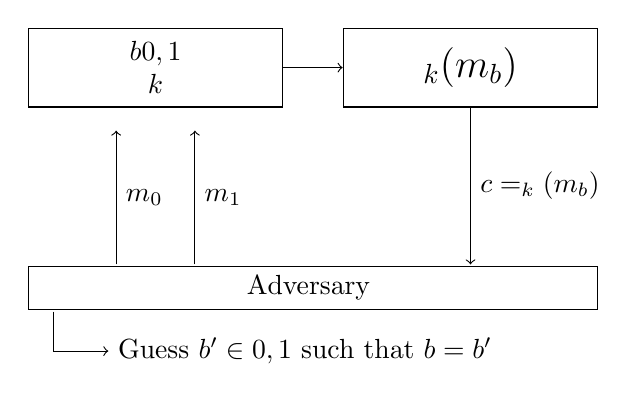
\begin{tikzpicture}[scale=1]
	\tikzstyle{BC} = [
	draw, rectangle,
	node distance=10pt,
	minimum width=3cm, minimum height=1cm,
	text width=3cm,
	align=center,
	]
	\tikzstyle{adv} = [
	draw, rectangle,
	node distance=10pt,
	minimum width=3cm, minimum height=0.5cm,
	text width=7cm,
	align=center,
	]
	
	\node[adv] at (2,-3.3+0.5) {Adversary $\adversary$};  
	\draw[->] (-.5,-2.5) -- node[right] {$m_0$} ++(0,+1.7);
	\draw[->] (.5,-2.5) -- node[right] {$m_1$} ++(0,+1.7);
	
	\node[BC] (b) at (0,0) {$b\uniform\set{0,1}$\\$k\uniform\keyspace$};
	\node[BC] (enc) at (4,0) {\Large{$\enc_{k}(m_b)$}};
	
	\draw[->] (b) -- (enc);
	
%	\draw[->] (4-0.5,-3+0.5) -- node[left] {$m$} ++(0,+2);
	\draw[->] (4,-0.5) 
	-- node[right] {$c=\enc_{k}(m_b)$} ++(0,-2);
	\draw[->] (-1.3,-3.1) 
	-- ++(0,-0.5) 
	-- ++(0.7,0) node[right] {Guess $b'\in\set{0,1}$ such that $b=b'$};
\end{tikzpicture}
\end{center}
The scheme is secure if the adversary's advantage is negligible: \[
\Adv_{\Pi}^{\text{IND-CPA}}(\adversary):=\abs{\Pr[b'=b]-\frac{1}{2}}\leq\negl(\lambda),
\] where $\lambda$ is the security parameter.
\end{example}

\newpage
\subsection{Perfect Security}
\begin{note}[Measure Theory]
Let $(\Omega,\mathcal{F}, \Pr)$ be a probability space, where: \begin{itemize}
	\item $\Omega$ is the sample space representing all possible outcomes.
	\item $\mathcal{F}$ is a $\sigma$-algebra of subsets of $\Omega$, representing the events.
	\item $\Pr:\mathcal{F}\to\intcc{0,1}$ is a probability measure satisfying $\Pr[\Omega]=1$.
\end{itemize}
\end{note}
\begin{note}[Random Variables]
\ \begin{itemize}
	\item A \textbf{plaintext random variable} $X:\Omega\to\plaintext$ is a measurable function, \ie, \[
	X^{-1}[A]\in\mathcal{F},\quad\forall A\subseteq\plaintext,\ \text{where $A$ is measurable}.
	\] This means $X$ maps outcomes in $\Omega$ to plaintexts in a way consistent with the probability structure. The distribution of $X$, denoted $P_X$, is the pushforward measure of $P$ under $X$:
	\[P_X(A)=P(X\in A)=P(\set{\omega\in\Omega:X(\omega)\in A}),\]
	for all measurable subsets $A\subseteq\plaintext$.	
	\item A \textbf{ciphertext random variable} $Y:\Omega\to\ciphertext$ is a measurable function, \ie, \[
	Y^{-1}[B]\in\mathcal{F},\quad\forall B\subseteq\ciphertext,\ \text{where $B$ is measurable}.
	\] This means $Y$ maps outcomes in $\Omega$ to ciphertexts in a measurable way. The distribution of $Y$, denoted $P_Y$, is the pushforward measure of $P$ under $Y$:
	\[P_Y(B)=P(Y\in B)=P(\set{\omega\in\Omega:Y(\omega)\in B}),\]
	for all measurable subsets $B\subseteq\ciphertext$.	
	\item A \textbf{random variable for the key space} $K:\Omega\to\keyspace$ is a measurable function, \ie, \[
	K^{-1}[A]\in\mathcal{F},\quad\forall A\subseteq\keyspace,\ \text{where $K$ is measurable}.
	\] This means $K$ maps outcomes in the sample space $\Omega$ to keys in 
	$\keyspace$ in a way consistent with the probability structure. The distribution of $K$, denoted $P_K$, is the pushforward measure of $P$ under $K$:
	\[P_K(A)=P(K\in A)=P(\set{\omega\in\Omega:K(\omega)\in A}),\]
	for all measurable subsets $A\subseteq\keyspace$.	
\end{itemize}
\end{note}
\begin{note}
	If the key is selected uniformly from $\keyspace$, then $P_K(A)$ is proportional to the size of $A$: \[
	P_K(A)=\frac{\abs{A}}{\abs{\keyspace}},\quad\forall A\subseteq\keyspace.
	\]
\end{note}

\defbox[Perfect Security of an Encryption Scheme]{\begin{definition}
	An encryption scheme $\Pi=(\keygen,\enc,\dec)$ is \textbf{perfect security} if, for every $m\in\messagespace$, $c\in\ciphertext$, and $k\in\keyspace$ such that $\enc(k,m)=c$, the following holds: \begin{enumerate}[(i)]
		\item \textbf{Ciphertext Independence}: \[
		\Pr[M=m\mid C=c]=\Pr[M=m],
		\] where 
		\begin{itemize}
			\item $M$ is the random variable representing the plaintext.
			\item $C$ is the random variable representing the ciphertext.
		\end{itemize}
		\item \textbf{Key Uniformity}: The key $K$ must satisfy: \[
		\Pr[\enc(K,m)=c]=\Pr[C=c],
		\] for all $m\in\messagespace$, $c\in\ciphertext$, and uniformly random $K$.
	\end{enumerate}
\end{definition}}
\begin{remark}
\[\Pr[M=m\mid C=c]=\Pr[M=m]\iff\Pr[C=c\mid M=m]=\Pr[C=c]\]
\end{remark}

\newpage
\thmbox{\begin{theorem}
	Consider a cryptosystem $(\plaintext,\ciphertext,\keyspace,\encryption,\decryption)$ where \[
	\abs{\plaintext}=\abs{\ciphertext}=\abs{\keyspace}.
	\] Then the cryptosystem (or encryption scheme) has perfect security if and only if \begin{enumerate}[(i)]
		\item every key is used with equal probability $1 /\ \abs{\keyspace}$, and
		\item $\forall x\in\plaintext,\ \forall y\in\ciphertext,\ \exists! k\in\keyspace\ \text{such that}\ \encryption_k(x)=y$.
	\end{enumerate}
\end{theorem}}
\begin{proof}
\begin{enumerate}
	\item[($\Rightarrow$)] By definition of perfect security, \[
	\Pr[X=x\mid Y=y]=\Pr[X=x],\quad\forall x\in\plaintext,\ y\in\ciphertext.
	\] 
	\begin{enumerate}[(i)]
		\item Let $K$ be the random variable representing the key. Since the ciphertext 
		$y$ is determined by the key $k$ and the plaintext $x$, we have: \[
		\Pr[Y=y\mid X=x]=\Pr[\exists k\in\keyspace\ \text{such that}\ \encryption_k(x)=y].
		\] To achieve uniform distribution of $Y$ for any fixed $x$, every key must be equality likely: \[
		\Pr[K=k]=\frac{1}{\abs{\keyspace}},\quad\forall k\in\keyspace.
		\]
		\item Assume that there exists two distinct keys $k_1,k_2\in\keyspace$, with $k_1\neq k_2$, such that \[
		\encryption_{k_1}(x)=y=\encryption_{k_2}(x),
		\] for some $x\in\plaintext$ and $y\in\ciphertext$.
		
		TBA
	\end{enumerate}
	\item[($\Leftarrow$)] Using Bayes' Theorem: \[
	\Pr[X=x\mid Y=y]=\frac{\Pr[Y=y\mid X=x]\Pr[X=x]}{\Pr[Y=y]}.
	\]
\end{enumerate}
\end{proof}

\newpage
\begin{example}[One-Time Pad]
The one-time pad encryption scheme is perfect security. \begin{itemize}
	\item $\messagespace=\ciphertext=\keyspace=\set{0,1}^n$;
	\item $\enc(k,m)=m\oplus k$, where $\oplus$ is bitwise XOR;
	\item $\dec(k,c)=c\oplus k$.
\end{itemize} We must show that $\Pr[C=c\mid M=m]=\Pr[C=c]$. For $m\in\messagespace$ and $c\in\ciphertext$, \begin{align*}
\Pr[C=c\mid M=m]&=\sum_{k\in\keyspace}\Pr[K=k]
\end{align*}
\end{example}
\newpage
\begin{center}
\begin{tikzpicture}[scale=1]
	\tikzstyle{XOR} = [
	line width=.25mm,
	draw,
	circle,
	outer sep=2pt,
	append after command={
		[shorten >=2bp, shorten <=2bp]
		(\tikzlastnode.north) edge[line width=.25mm] (\tikzlastnode.south)
		(\tikzlastnode.east) edge[line width=.25mm] (\tikzlastnode.west)}
	]
	
	\node[draw, rectangle] (pt) {Plaintext};  
	\node[XOR, right=1cm of pt] (xor) {};
	\node[draw, rectangle, above=2cm of xor] (mask) {$k\uniform\keyspace$};
	\node[draw, rectangle, right=1cm of xor] (ct) {Ciphertext};  
	
	\draw[-{Latex}] (pt) to (xor);
	\draw[-{Latex}] (xor) to (ct);
	\draw[-{Latex}] (mask) -- node[right] {mask} ++(0,-2.5);
	\begin{scope}[xshift=8cm]
	\node[draw, rectangle] (pt) {$\cdots$\texttt{10101010}};  
	\node[XOR, right=1cm of pt] (xor) {};
	\node[draw, rectangle, above=2cm of xor] (mask) {\textcolor{red}{$\cdots$\texttt{11110000}} $\uniform\set{0,1}^n$};
	\node[draw, rectangle, right=1cm of xor] (ct) {\color{magenta}$\cdots$\texttt{10100000}};  
	
	\draw[-{Latex}] (pt) to (xor);
	\draw[-{Latex}] (xor) to (ct);
	\draw[-{Latex}] (mask) -- node[right] {mask} ++(0,-2.5);
	\end{scope}
\end{tikzpicture}
\end{center}
\thmbox{\begin{theorem}
	The one-time pad encryption scheme is perfectly secret.
\end{theorem}}
\begin{proof}
\begin{align*}
	\Pr[C=c\mid M=m]=\Pr[c=\enc(K,m)]&=\Pr[c=m\oplus K]\\
	&=\Pr[K=m\oplus c]\\
	&=2^{-n}\quad\text{if}\ K\uniform\keyspace=\set{0,1}^n
\end{align*} Fix any distribution over $\messagespace$. For any $c\in\ciphertext$, we have \begin{align*}
\Pr[C=c]&=\sum_{m\in\messagespace}\Pr[C=c\mid M=m]\cdot\Pr[M=m]\\
&=2^{-n}\cdot\Pr[M=m]
\end{align*} By Bayes' Theorem, we obtain \begin{align*}
\Pr[M=m\mid C=c]&=\frac{\Pr[C=c\mid M=m]\cdot\Pr[M=m]}{\Pr[C=c]}\\
&=\frac{2^{-n}\cdot\Pr[M=m]}{2^{-n}}\\
&=\Pr[M=m].
\end{align*}
\end{proof}